%%%%%%%%%%%%%%%%%%%%%%%%%%%%%%%%%%%%%%%%%%%%%%%%%%%%%%%%%%%%%%%%%%%%%%%%
%    INSTITUTE OF PHYSICS PUBLISHING                                   %
%                                                                      %
%   `Preparing an article for publication in an Institute of Physics   %
%    Publishing journal using LaTeX'                                   %
%                                                                      %
%    LaTeX source code `ioplau2e.tex' used to generate `author         %
%    guidelines', the documentation explaining and demonstrating use   %
%    of the Institute of Physics Publishing LaTeX preprint files       %
%    `iopart.cls, iopart12.clo and iopart10.clo'.                      %
%                                                                      %
%    `ioplau2e.tex' itself uses LaTeX with `iopart.cls'                %
%                                                                      %
%%%%%%%%%%%%%%%%%%%%%%%%%%%%%%%%%%
%
%
% First we have a character check
%
% ! exclamation mark    " double quote  
% # hash                ` opening quote (grave)
% & ampersand           ' closing quote (acute)
% $ dollar              % percent       
% ( open parenthesis    ) close paren.  
% - hyphen              = equals sign
% | vertical bar        ~ tilde         
% @ at sign             _ underscore
% { open curly brace    } close curly   
% [ open square         ] close square bracket
% + plus sign           ; semi-colon    
% * asterisk            : colon
% < open angle bracket  > close angle   
% , comma               . full stop
% ? question mark       / forward slash 
% \ backslash           ^ circumflex
%
% ABCDEFGHIJKLMNOPQRSTUVWXYZ 
% abcdefghijklmnopqrstuvwxyz 
% 1234567890
%
%%%%%%%%%%%%%%%%%%%%%%%%%%%%%%%%%%%%%%%%%%%%%%%%%%%%%%%%%%%%%%%%%%%
%
\renewcommand{\theequation}{\arabic{equation}}
\newtheorem{lemma}{Lemma}

\documentclass[12pt]{iopart}

\usepackage{braket}

\usepackage{amsthm}

\usepackage[
backend=biber,
style=numeric-comp,
sorting=none
]{biblatex}

\addbibresource{main/bibliography.bib}
\usepackage{graphicx}
\usepackage{amsmath}
\newcommand{\gguide}{{\it Preparing graphics for IOP Publishing journals}}
%Uncomment next line if AMS fonts required
%\usepackage{iopams}  


\begin{document}
\begin{center}
    {\Large \textbf{Supplementary Information}}\\[2ex]
\end{center}
\setcounter{equation}{0}


%
% Uncomment for keywords
%\vspace{2pc}
%\noindent{\it Keywords}: XXXXXX, YYYYYYYY, ZZZZZZZZZ
%
% Uncomment for Submitted to journal title message
%\submitto{\JPA}
%
% Uncomment if a separate title page is required
%\maketitle
% 
% For two-column output uncomment the next line and choose [10pt] rather than [12pt] in the \documentclass declaration
%\ioptwocol
%


\section*{Appendix A}


\textit{Lemma A1.} If an X or CX gate $g$ may be applied to a pattern $p$, then for all quantum
    states $\ket{x}$, $g\xi_p\ket{x} = \xi_{g(p)}g\ket{x}$, \forall g \in  \{ X(i), CX(i,j) \vert p_i\neq*, p_j\neq* \}$
\begin{proof}


Define $g(i)$ such that $g\ket{i} = \ket{g(i)}$. Then $g(i) \in I_{g(p)}$ for all
$i \in I_p$. This also implies $g(g(i)) \in I_{g(g(p))}$ for all $g(i) \in I_{g(p)}$.
Applying $g$ twice amounts to the identity transformation in the
context of both patterns and substates, thus, $i \in I_p$ for all $g(i) \in I_{g(p)}$,
implying that $g$ creates a bijection between $I_p$ and $I_{g(p)}$. In addition, given
that X and CX gates on quantum states represent amplitude permutations in the
computational basis, $\braket{g(i)|g|x} = \braket{i|x}$.  It then follows that,
\begin{align}
\label{eq6}
  g\xi_p\ket{x} &= g\sum_{i \in I_p}{{\ket{i}}{\braket{i|x}}} \nonumber \\
  &= \sum_{i \in I_p}{{\ket{g(i)}}{\braket{i|x}}} \nonumber \\
  &= \sum_{i \in I_p}{{\ket{g(i)}}{\braket{g(i)|g|x}}} \nonumber \\
  &= \sum_{j \in I_{g(p)}}{{\ket{j}}{\braket{j|g|x}}} \nonumber \\
  &= \xi_{g(p)}g\ket{x}
\end{align}
\end{proof}

\section*{Appendix B: Refinements for the ISA method}
We describe two optimizations to our implementation of the ISA framework:
refinement by RZ-RY, and retroactive base case reduction.

\subsection*{B.1. Refinement by RZ-RY}
Refinement by RZ-RY seeks to apply approximate quantum state preparation to the
target state $\ket{x}$ without using any CX gates, before applying the ISA
framework. This is done by selecting a zero-bit pattern $p$ such that
$\| \xi_p\ket{x} \|$ is maximized (ties are broken randomly), then applying substate
merging several times to eventually merge $\xi_p\ket{x}$ into $\xi_{p'}\ket{x}$. The
selection procedure resembles the implementation of prepare, but using substate
merging instead of controlled substate merging:
\begin{enumerate}
\item If $p$ is the string of all zeroes, then terminate this procedure.
Otherwise, continue.
\item Construct the set $P$, containing zero-bit patterns $p'$ that differ from
$p$.
\item Select $p'$ such that $\xi_{p'}\ket{x}$ is maximized, with ties broken
randomly.
\item Let $i$ be the index where $p$ and $p'$ differ. If $p[i] = 0$ then merge
$\xi_{p'}\ket{x}$ into $\xi_p\ket{x}$, otherwise, merge $\xi_p\ket{x}$ into $\xi_{p'}\ket{x}$
and update $p = p'$. Return to step 1.
\end{enumerate}

\begin{figure}[h]
\centering
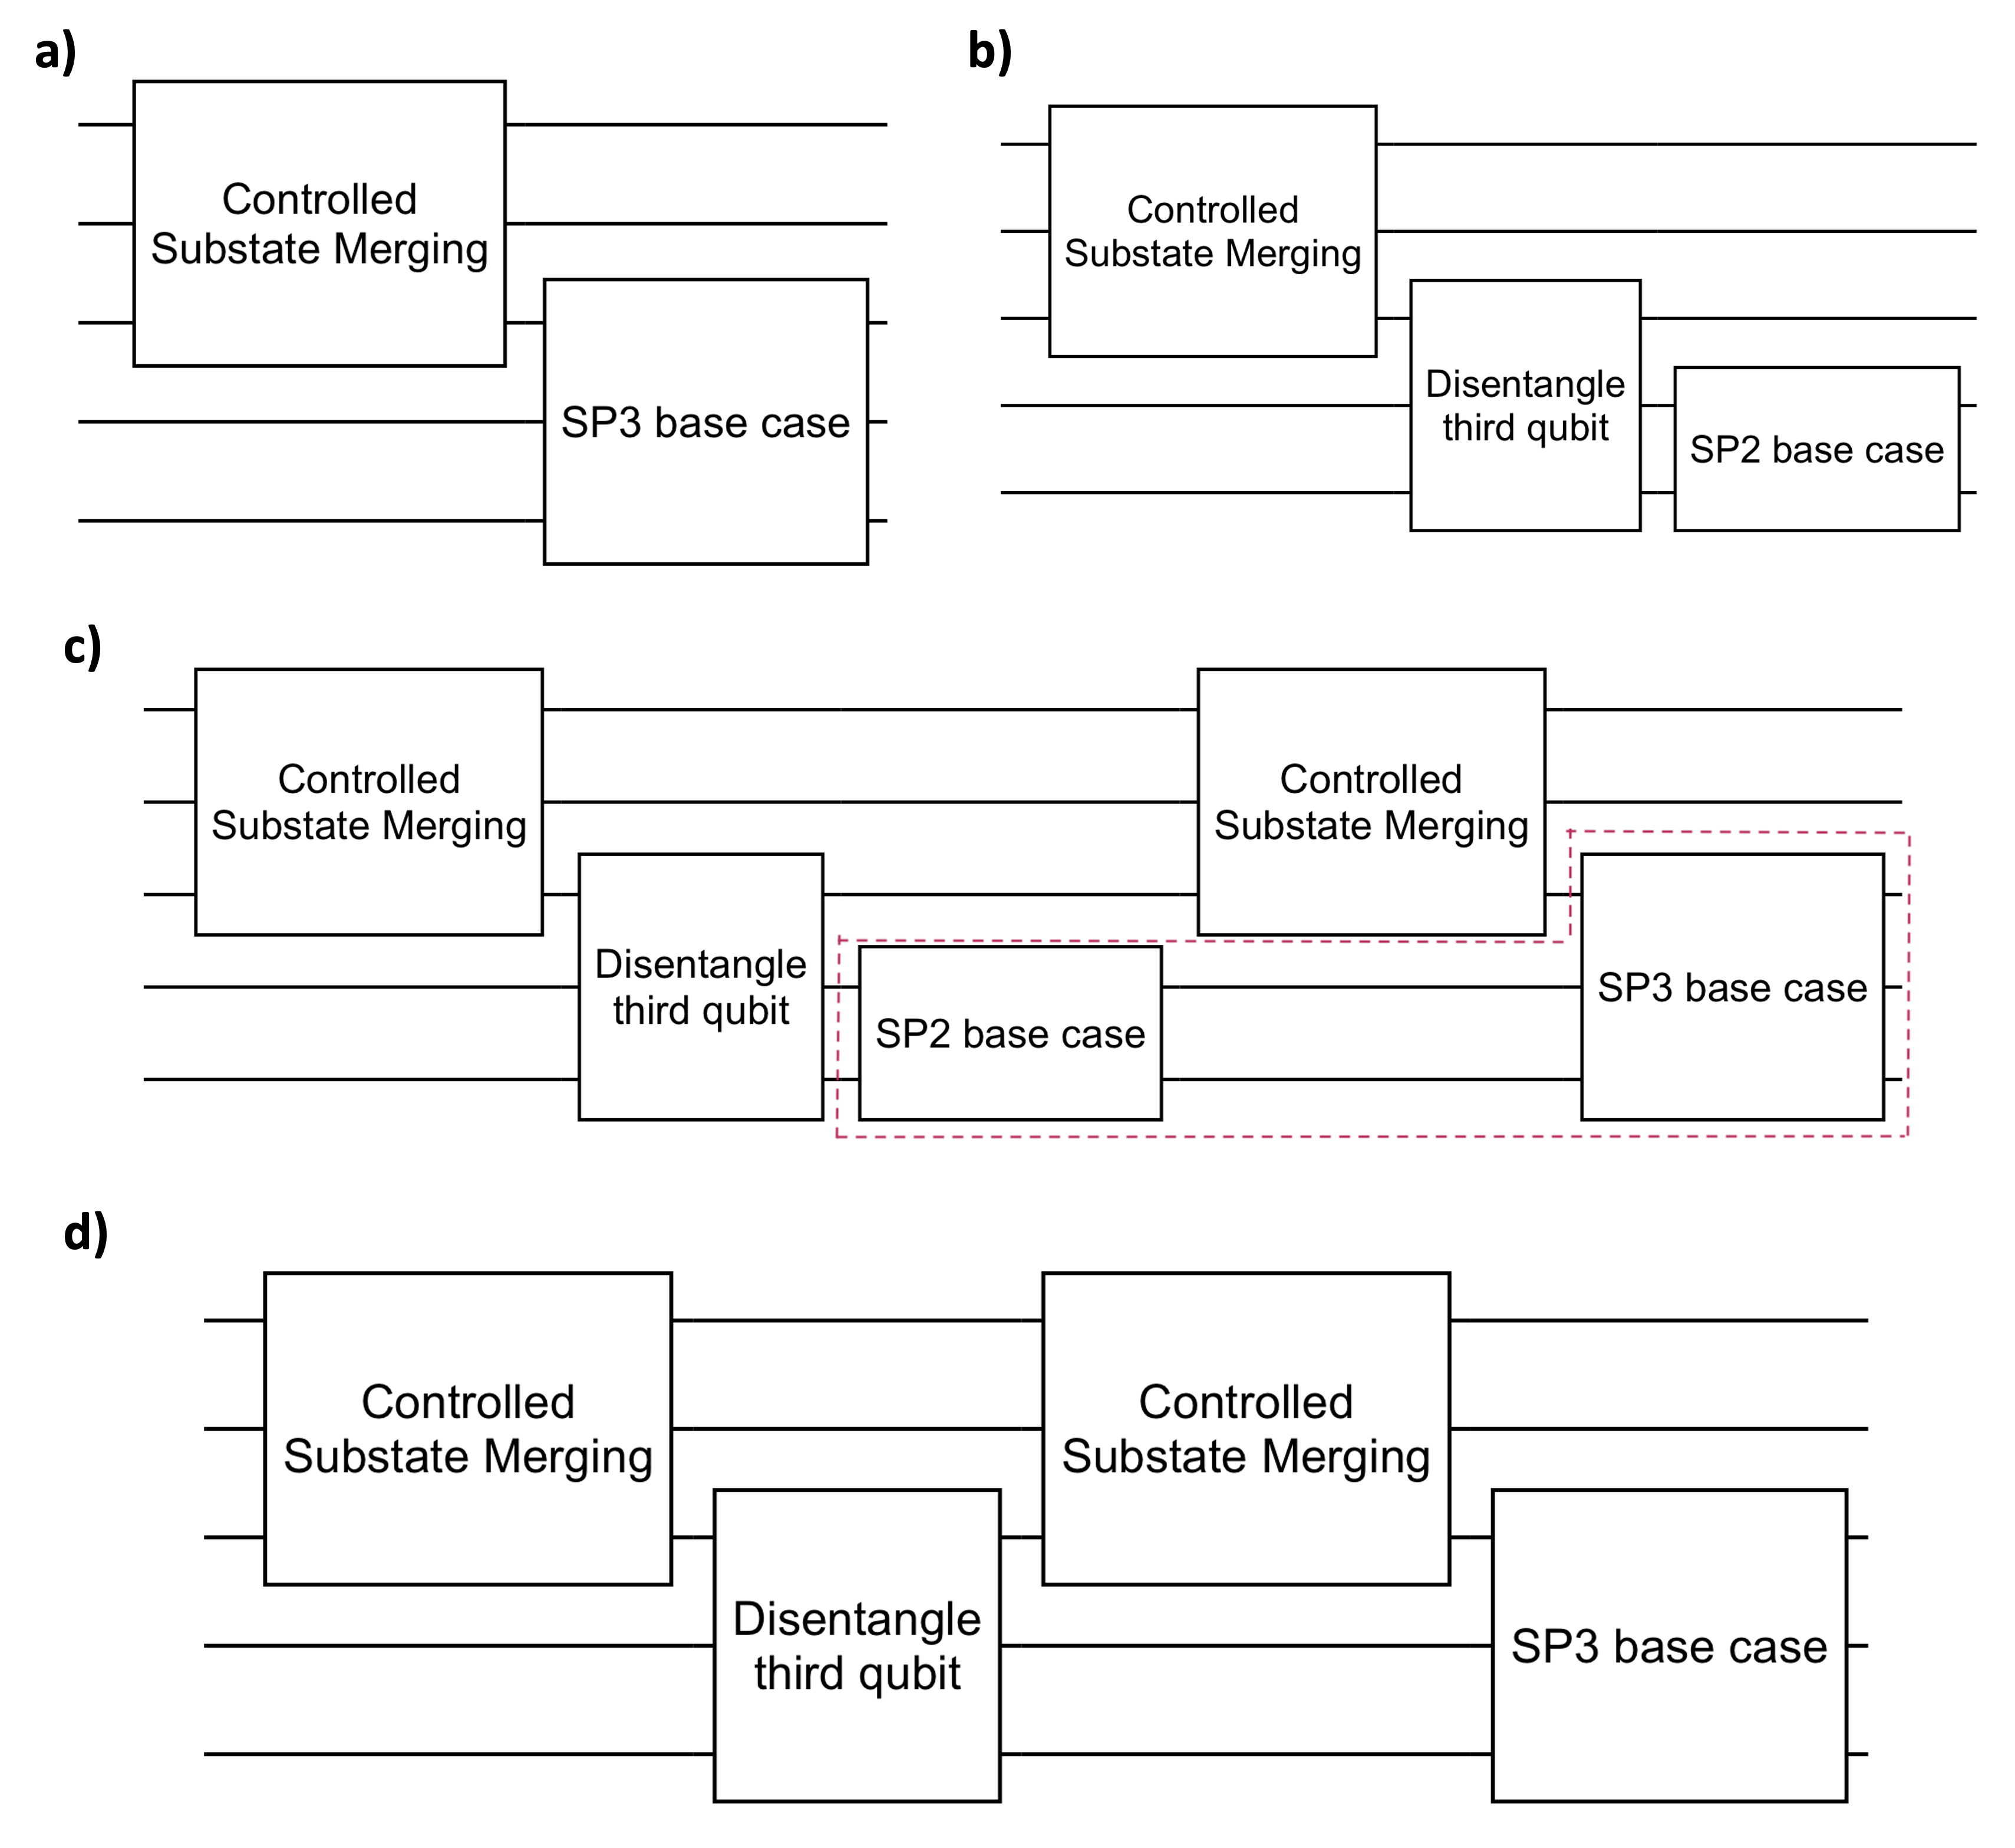
\includegraphics[width=0.95\linewidth]{main/figs/sfig_1.png}
\caption{Quantum circuit components comprising the ISA framework. a) General quantum circuit structure of a single iteration of ISA using a
two-bit pattern $p$. Several iterations of controlled substate merging are
performed on neighboring qubits before a three-qubit state preparation base case
is applied. b) Decomposition of a single iteration of ISA using a two-bit pattern $p$.
The three-qubit state preparation base case is broken down into a distangling
step and a two-qubit state preparation base case. c) General quantum circuit structure for two consecutive iterations of ISA
ending in a three-qubit base case on the same three qubits. Note that the SP2 
base case in the first ISA iteration can be commuted with the controlled substate
merging step in the second ISA iteration. d) General quantum circuit structure for two consecutive iterations of ISA
width the same three-qubit state preparation base case after applying retroactive
base case reduction. The SP2 block from Figure 4 is merged with the later SP3
block, saving 1 CX gate.}
\label{sfig1}
\end{figure}

\subsection*{B.2. Retroactive Base Case Reduction}
When a two-bit pattern $p$ is chosen in the select step, the corresponding quantum
circuit takes on the structure shown in Figure \ref{sfig1}a. The three-qubit QSP step can be broken into two steps: disentangling the third 
qubit and two-qubit state preparation on the remaining two qubits, as shown in 
Figure \ref{sfig1}b. However, if two consecutive iterations of ISA both selected a
two-bit pattern and those 
two patterns had their `$*$' characters on the same two qubits, the resulting 
quantum circuit would have the structure shown in Figure \ref{sfig1}c. Then,
the part of the quantum circuit enclosed in dotted lines first performs 
two-qubit state preparation on the lower two qubits, then performs three-qubit 
state preparation on all three relevant qubits. These two transformations have 
the net effect of transforming the three-qubit substate to $\ket{\mathbf{0}}$ and can
instead be replaced by a single three-qubit state preparation routine. This
procedure saves the one CX gate used by the two-qubit state preparation base
case.

\section*{Appendix C: Optimal, exact three-qubit state preparation}
Optimal, exact three-qubit state preparation has been studied in the 
literature \cite{PhysRevA.77.032320}; our specific implementation requires
three steps, called ``D1'', ``D2'', and ``SP2''. Let the target state be
\begin{equation}
\ket{x} = \sum_{i, j, k \in \{0, 1\}}{a_{ijk}\ket{ijk}}.
\end{equation}
Step D1 applies a single-qubit rotation, then CX(0, 1), then another single-qubit
rotation, resulting in the state
\begin{equation}
\ket{y} = \sum_{i, j, k \in \{0, 1\}}{b_{ijk}\ket{ijk}},
\end{equation}
such that
\begin{equation}
\frac{b_{110}}{b_{010}} = \frac{b_{111}}{b_{011}} \quad 
  and \quad \frac{b_{100}}{b_{000}} = \frac{b_{101}}{b_{001}}.
\end{equation}
Next, step D2 uses a single-qubit rotation, CX(1, 2), and another single-qubit
rotation to transform $\ket{y}$ into a two-qubit state
\begin{equation}
\ket{z} = \sum_{j, k \in \{0, 1\}}{c_{jk}\ket{0jk}}.
\end{equation}
Finally, step SP2 implements two-qubit state preparation on this state using one
CX gate and several single-qubit rotations. We describe each of these steps in detail,
starting with SP2 and D2. Then, we briefly discuss the decomposition of uniformly
controlled single-qubit rotations before concluding with a description of D1.

\subsection*{C.1. SP2}
Starting from the state 
\begin{equation}
\ket{z} = \sum_{j, k \in \{0, 1\}}{c_{jk}\ket{0jk}},
\end{equation}
we rotate merge $c_{001}\ket{001}$ into $c_{000}\ket{000}$, leading to the state:
\begin{equation}
\ket{z'} = c'_{000}\ket{000} + c'_{010}\ket{010} + c'_{011}\ket{011}.
\end{equation}
Next, $c'_{011}\ket{011}$ is controlled rotate merged into $c'_{010}\ket{010}$. This
results in a one-qubit state that can be prepared using a single-qubit rotation gate.

\subsection*{C.2. Step D2}
Starting from the state
\begin{equation}
\ket{y} = \sum_{i, j, k \in \{0, 1\}}{b_{ijk}\ket{ijk}},
\end{equation}
 we rotate merge $b_{100}\ket{100}$ into $b_{000}\ket{000}$. The pre-condition
\begin{equation}
\frac{b_{100}}{b_{000}} = \frac{b_{101}}{b_{001}}
\end{equation}
ensures that this procedure also merges $b_{101}\ket{101}$ into $b_{001}\ket{001}$.
This results in the state:
\begin{align}
\ket{y} = \sum_{i, j, k \in \{0, 1\}}{b'_{ijk}\ket{ijk}} \nonumber \\
\text{such that} \quad b'_{100}, b'_{101} = 0
\end{align}
In addition, the RZ and RY gate were applied to qubit 2, therefore, the equality
\begin{equation}
\frac{b_{110}}{b_{010}} = \frac{b_{111}}{b_{011}}
\end{equation}
is preserved after the transformation.
\begin{equation}
\frac{b'_{110}}{b'_{010}} = \frac{b'_{111}}{b'_{011}}
\end{equation}
Next, $b'_{110}\ket{110}$ is controlled rotate merged into $b'_{010}\ket{010}$. The
equality
\begin{equation}
\frac{b'_{110}}{b'_{010}} = \frac{b'_{111}}{b'_{011}}
\end{equation}
ensures that $b'_{111}\ket{111}$ is also merged into $b'_{011}\ket{011}$ by this
process. The previous step zeroed out the $\ket{100}$ and $\ket{101}$ basis vectors;
this step zeroed out the $\ket{110}$ and $\ket{111}$ basis vectors. Therefore, the
result of these transformations is a two-qubit state:
\begin{equation}
\ket{z} = \sum_{j, k \in \{0, 1\}}{c_{jk}\ket{0jk}}.
\end{equation}
\subsection*{C.3. Decomposing Uniformly Controlled Single-Qubit Rotations}
In this section, we describe the set of uniformly controlled single-qubit rotations 
with one control qubit that can be decomposed into one CX gate and single-qubit 
rotations. In addition, we give a procedure for their decomposition. These 
constructions will be necessary for the construction of step D1 for optimal, exact 
three-qubit state preparation.

\begin{figure}[h]
\centering
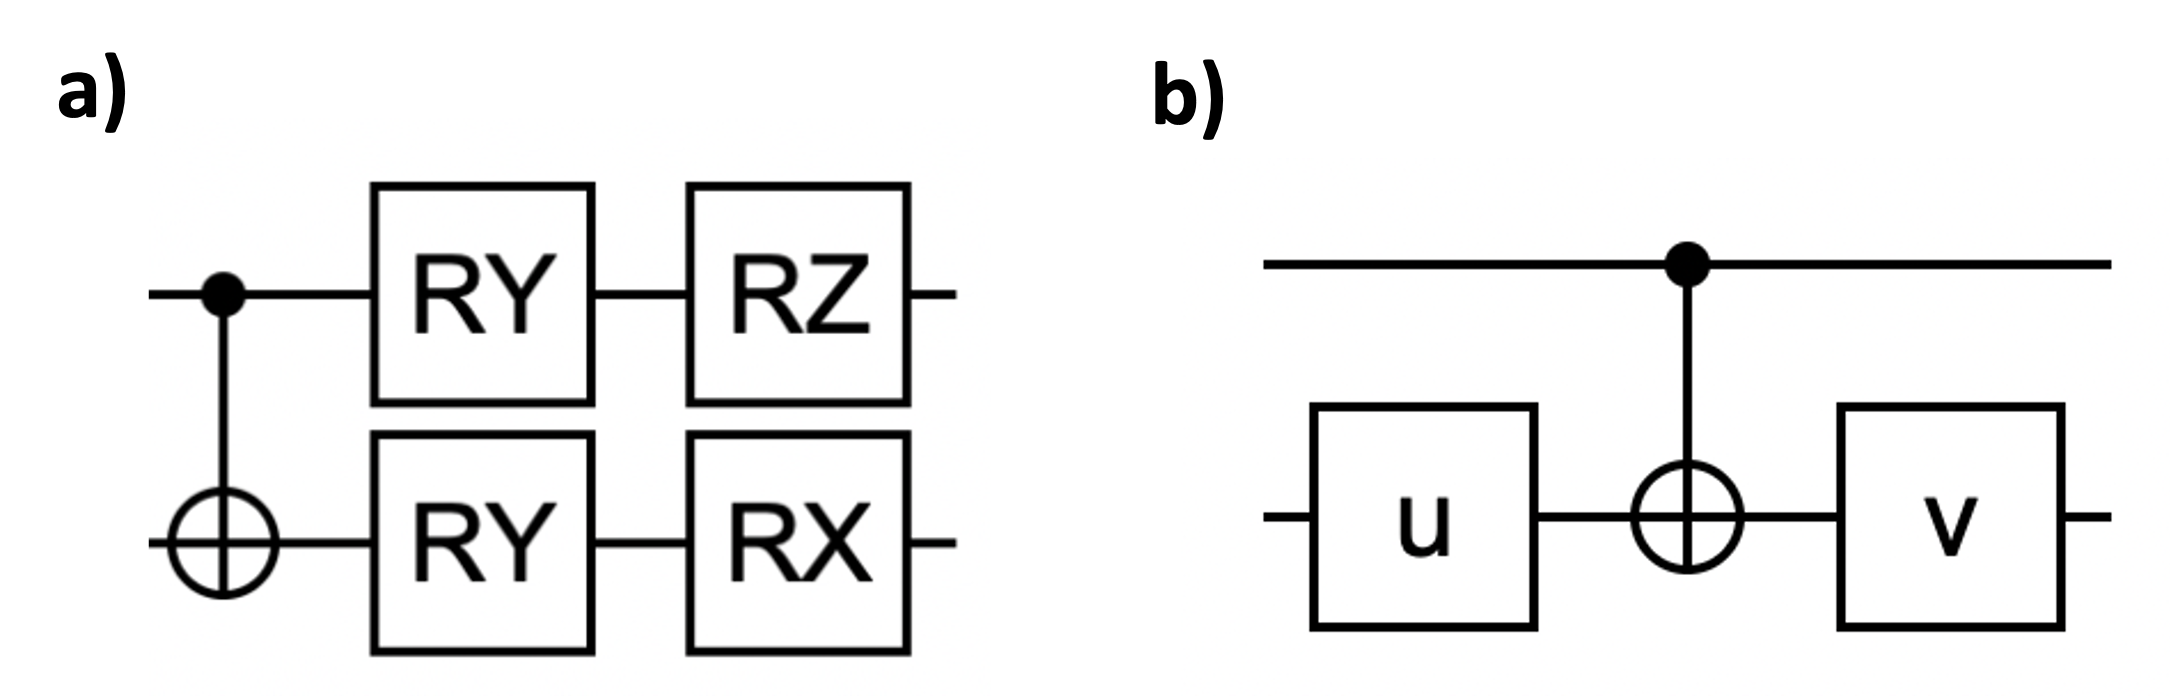
\includegraphics[width=0.6\linewidth]{main/figs/sfig_2.png}
\caption{a) The circuit block used in ADAPT-VQE for state preparation. The operator
pool was generated by translating this block across different pairs of 
adjacent qubits. Each operator contains four parameters, one for each rotation.
All four rotation angles were initialized to zero. b) Target decomposition of the uniformly controlled single-qubit rotation with one control qubit}
\label{sfig2}
\end{figure}

For simplicity, let the control qubit be qubit 1, let the target qubit be qubit 0. 
Suppose the desired gate applies $a$ if the control qubit is 0, applies $b$ 
otherwise. Then the desired gate has matrix form 
\begin{equation}
\begin{bmatrix}a&0\\0&b\end{bmatrix}.
\end{equation}
We wish to decompose this transformation into a quantum circuit of the form shown in
Figure \ref{sfig2}b.




These gates, together, take the matrix form
\begin{equation}
\begin{bmatrix}v&0\\0&v\end{bmatrix}
\begin{bmatrix}I&0\\0&X\end{bmatrix}
\begin{bmatrix}u&0\\0&u\end{bmatrix},
\end{equation}
This requires some $u$ and $v$ to exist such that $a = vu$ and $b = vXu$. Then
\begin{equation}
ab^\dagger = (vu)(vXu)^\dagger = vXv^\dagger,
\end{equation}
which implies that $ab^\dagger$ must have the same eigenvalues, $\pm 1$, as $X$.
This condition is both necessary and sufficient for the uniformly controlled rotation
to be decomposable into the quantum circuit shown. Indeed, if $ab^\dagger$ has the
same eigenvalues as $X$, then we can compute $v$ by diagonalization, then compute
$u = v^\dagger a$. Finally, $u$ and $v$ can be decomposed to RY and RZ gates using
ZYZ decomposition.

\subsection*{C.4. Step D1}
Step D1 is implemented using a uniformly controlled single-qubit rotation, with
qubit 0 as the control, qubit 1 as the target. To implement D1, we construct
single-qubit operations $a$ and $b$ such that applying
$\begin{bmatrix}a&0\\0&b\end{bmatrix}$ to $\ket{x}$ leads to the state
\begin{equation}
\ket{y} = \sum_{i, j, k \in \{0, 1\}}{b_{ijk}\ket{ijk}},
\end{equation}
such that
\begin{equation}
\frac{b_{110}}{b_{010}} = \frac{b_{111}}{b_{011}} 
  \text{ and } \frac{b_{100}}{b_{000}} = \frac{b_{101}}{b_{001}}
\end{equation}
In addition, we perform this construction such that $ab^\dagger$ has eigenvalues
$\pm 1$ to ensure the transformation can be implemented using only one CX gate.

We parameterize $a$ and $b$ as:
\begin{align}
a &= e^{i\phi_g}\begin{bmatrix}cos(\theta_a)&-sin(\theta_a)e^{i\phi_a}\\
  sin(\theta_a)e^{i\alpha_a}&cos(\theta_a)e^{i(\alpha_a + \phi_a)}\end{bmatrix} 
  \nonumber \\
b &= \begin{bmatrix}cos(\theta_b)&-sin(\theta_b)e^{i\phi_b}\\
  sin(\theta_b)e^{i\alpha_b}&cos(\theta_b)e^{i(\alpha_b + \phi_b)}\end{bmatrix}
\end{align}
Then, we can express the $b_{ijk}$ coefficients of $\ket{y}$ in terms of
$\phi_g$, $\theta_a$, $\alpha_a$, $\phi_a$, $\theta_b$, $\alpha_b$, $\phi_b$,
and the $a_{ijk}$ coefficients of $\ket{x}$:

\begin{align}
b_{000} &= e^{i\phi_g}(cos(\theta_a)a_{000} + sin(\theta_a)e^{i\phi_a}a_{010}) 
  \nonumber \\
b_{010} &= e^{i(\alpha_a + \phi_g)}(-sin(\theta_a)a_{000} +
  cos(\theta_a)e^{i\phi_a}a_{010}) \nonumber \\
b_{100} &= e^{i\phi_g}(cos(\theta_a)a_{100} + sin(\theta_a)e^{i\phi_a}a_{110}) 
  \nonumber \\
b_{110} &= e^{i(\alpha_a + \phi_g)}(-sin(\theta_a)a_{100} +
  cos(\theta_a)e^{i\phi_a}a_{110}) \nonumber \\
b_{001} &= cos(\theta_b)a_{001} + sin(\theta_b)e^{i\phi_b}a_{011} \nonumber \\
b_{011} &= e^{i\alpha_b}(-sin(\theta_b)a_{001} + cos(\theta_b)e^{i\phi_b}a_{011}) 
  \nonumber \\
b_{101} &= cos(\theta_b)a_{101} + sin(\theta_b)e^{i\phi_b}a_{111} \nonumber \\
b_{111} &= e^{i\alpha_b}(-sin(\theta_b)a_{101} + cos(\theta_b)e^{i\phi_b}a_{111})
  \nonumber \\
\end{align}
Then the constraints
\begin{equation}
\frac{b_{110}}{b_{010}} = \frac{b_{111}}{b_{011}} 
  \text{ and }\frac{b_{100}}{b_{000}} = \frac{b_{101}}{b_{001}}
\end{equation}
Can be written as:

\begin{align}
\frac{e^{i(\alpha_a + \phi_g)}(-sin(\theta_a)a_{100} + cos(\theta_a)e^{i\phi_a}a_{110})}{e^{i(\alpha_a + \phi_g)}(-sin(\theta_a)a_{000} + cos(\theta_a)e^{i\phi_a}a_{010})} &= 
\frac{e^{i\alpha_b}(-sin(\theta_b)a_{101} + cos(\theta_b)e^{i\phi_b}a_{111})}{e^{i\alpha_b}(-sin(\theta_b)a_{001} + cos(\theta_b)e^{i\phi_b}a_{011})} \nonumber \\
\frac{e^{i\phi_g}(cos(\theta_a)a_{100} + sin(\theta_a)e^{i\phi_a}a_{110})}{e^{i\phi_g}(cos(\theta_a)a_{000} + sin(\theta_a)e^{i\phi_a}a_{010})} &= \frac{cos(\theta_b)a_{101} + sin(\theta_b)e^{i\phi_b}a_{111}}
{cos(\theta_b)a_{001} + sin(\theta_b)e^{i\phi_b}a_{011}}
\end{align}

The $e^{i\alpha_a}$, $e^{i\alpha_b}$, $e^{i\phi_g}$ terms cancel out,
making $\phi_g$, $\alpha_a$, and $\alpha_b$ free parameters. Multiplying out
the denominators, dividing by $cos(\theta_a)cos(\theta_b)$, and re-arranging the
terms gives:

\begin{align}
Atan(\theta_a)tan(\theta_b) + Btan(\theta_a)e^{i\phi_b} + Ctan(\theta_b)e^{i\phi_a} + De^{i(\phi_a + \phi_b)} = 0 \nonumber \\
A - Btan(\theta_b)e^{i\phi_b} - Ctan(\theta_a)e^{i\phi_a} + Dtan(\theta_a)tan(\theta_b)e^{i(\phi_a + \phi_b)} = 0
\end{align}

where
\begin{align}
A &= a_{100}a_{001} - a_{000}a_{101}\nonumber \\
B &= a_{100}a_{011} - a_{000}a_{111}\nonumber \\
C &= a_{110}a_{001} - a_{010}a_{101}\nonumber \\
D &= a_{110}a_{011} - a_{010}a_{111}
\end{align}

Dividing the first equation by $e^{i(\phi_a + \phi_b)}$ and taking its conjugate
results in the following system of equations:

\begin{align}
A^*tan(\theta_a)tan(\theta_b)e^{i(\phi_a + \phi_b)} + B^*tan(\theta_a)e^{i\phi_a} + C^*tan(\theta_b)e^{i\phi_b} + D^* = 0 \nonumber \\
A - Btan(\theta_b)e^{i\phi_b} - Ctan(\theta_a)e^{i\phi_a} + Dtan(\theta_a)tan(\theta_b)e^{i(\phi_a + \phi_b)} = 0.
\end{align}

Performing the substitution
\begin{align}
x = tan(\theta_a)e^{i\phi_a} \nonumber \\
y = tan(\theta_b)e^{i\phi_b}
\end{align}

Results in the system of equations:
\begin{align}
A^*xy + B^*x + C^*y + D^* = 0 \nonumber \\
A - By - Cx + Dxy = 0
\end{align}

Which can be solved by substitution. Once $x$ and $y$ are known,
$\theta_a$, $\theta_b$, $\phi_a$, $\phi_b$ can be determined.

Next, the constraint on the eigenvalues of $ab^\dagger$ needs to be satisfied.
Using the same parameterization as before, we can write:
\begin{align}
a &= e^{i\phi_g}\begin{bmatrix}cos(\theta_a)&-sin(\theta_a)e^{i\phi_a}\\
  sin(\theta_a)e^{i\alpha_a}&cos(\theta_a)e^{i(\phi_a + \alpha_a)}\end{bmatrix}
  = e^{i\phi_g}\begin{bmatrix}1&0\\0&e^{i\alpha_a}\end{bmatrix}\begin{bmatrix}
  cos(\theta_a)&-sin(\theta_a)e^{i\phi_a}\\sin(\theta_a)&cos(\theta_a)e^{i\phi_a}
  \end{bmatrix} \nonumber \\
b &= \begin{bmatrix}cos(\theta_b)&-sin(\theta_b)e^{i\phi_b}\\
  sin(\theta_b)e^{i\alpha_b}&cos(\theta_b)e^{i(\phi_b + \alpha_b)}\end{bmatrix}
  = \begin{bmatrix}1&0\\0&e^{i\alpha_b}\end{bmatrix}\begin{bmatrix}cos(\theta_b)
  &-sin(\theta_b)e^{i\phi_b}\\sin(\theta_b)&cos(\theta_b)e^{i\phi_b}\end{bmatrix}
  \nonumber \\
ab^\dagger &= e^{i\phi_g}\begin{bmatrix}1&0\\0&e^{i\alpha_a}\end{bmatrix}\left(
  \begin{bmatrix}cos(\theta_a)&-sin(\theta_a)e^{i\phi_a}\\
  sin(\theta_a)&cos(\theta_a)e^{i\phi_a}\end{bmatrix}\begin{bmatrix}
  cos(\theta_b)&-sin(\theta_b)e^{i\phi_b}\\sin(\theta_b)
  &cos(\theta_b)e^{i\phi_b}\end{bmatrix}^\dagger\right)\begin{bmatrix}1&0\\
  0&e^{i\alpha_b}\end{bmatrix}^\dagger \label{abt}
\end{align}

The two matrices between the parentheses in Eq. (\ref{abt}) are unitary matrices, thus, their
product is a unitary matrix and can be expressed as
\begin{equation}
\begin{bmatrix}cos(\theta_a)&-sin(\theta_a)e^{i\phi_a}\\
  sin(\theta_a)&cos(\theta_a)e^{i\phi_a}\end{bmatrix}\begin{bmatrix}
  cos(\theta_a)&-sin(\theta_a)e^{i\phi_a}\\sin(\theta_a)
  &cos(\theta_a)e^{i\phi_a}\end{bmatrix}^\dagger = 
  e^{i\alpha_g}\begin{bmatrix}cos(\theta)&-sin(\theta)e^{i\phi}\\
  sin(\theta)e^{i\alpha}&cos(\theta)e^{i(\alpha + \phi)}\end{bmatrix}
\end{equation}
for some $\alpha_g$, $\alpha$, $\phi$, and $\theta$. Then, we can write
\begin{align}
ab^\dagger &= e^{i\phi_g}\begin{bmatrix}1&0\\0&e^{i\alpha_a}\end{bmatrix}
  e^{i\alpha_g}\begin{bmatrix}cos(\theta)&-sin(\theta)e^{i\phi}\\
  sin(\theta)e^{i\alpha}&cos(\theta)e^{i(\alpha + \phi)}\end{bmatrix}
  \begin{bmatrix}1&0\\0&e^{i\alpha_b}\end{bmatrix}^\dagger \nonumber \\
 &= e^{i(\phi_g + \alpha_g)}\begin{bmatrix}cos(\theta)&-sin(\theta)
  e^{i(\phi - \alpha_b)}\\sin(\theta)e^{i(\alpha + \alpha_a)}
  &cos(\theta)e^{i(\phi + \alpha + \alpha_a - \alpha_b)}\end{bmatrix}
\end{align}

The characteristic polynomial of this matrix is:
\begin{align}
p(t) &= (cos(\theta)e^{i(\phi_g + \alpha_g)} - t)
(cos(\theta)e^{i(\phi + \alpha + \alpha_a - \alpha_b + \phi_g + \alpha_g)} - t) \nonumber \\
&\quad \quad - (-sin(\theta)e^{i(\phi - \alpha_b + \phi_g + \alpha_g)})
  (sin(\theta)e^{i(\alpha - \alpha_a + \phi_g + \alpha_g)}) \nonumber \\
 &= t^2 - e^{i(\phi_g + \alpha_g)}cos(\theta)(1 + e^{i(\phi + \alpha + \alpha_a - \alpha_b)})t 
  + cos(\theta)^2e^{i(2(\phi_g + \alpha_g) + \phi + \alpha + \alpha_a - \alpha_b)} \nonumber \\
  &\quad \quad+ sin(\theta)^2e^{i(2(\phi_g + \alpha_g) + \phi + \alpha + \alpha_a - \alpha_b)} \nonumber \\
 &= t^2 - e^{i(\phi_g + \alpha_g)}cos(\theta)(1 + e^{i(\phi + \alpha + \alpha_a - \alpha_b)})t + e^{2i(\phi_g + \alpha_g)}e^{i(\phi + \alpha + \alpha_a - \alpha_b)}
\end{align}
We require the eigenvalues to be $\pm 1$, so the characteristic polynomial must
be equal to $t^2 - 1$. This requires:
\begin{align}
e^{i(\phi_g + \alpha_g)}cos(\theta)(1 + e^{i(\phi + \alpha + \alpha_a - \alpha_b)}) = 0 \nonumber \\
e^{2i(\phi_g + \alpha_g)}e^{i(\phi + \alpha + \alpha_a - \alpha_b)} = -1
\end{align}
Solving these equations gives:
\begin{align}
\phi + \alpha + \alpha_a - \alpha_b = \pi \nonumber \\
\phi_g + \alpha_g = 0
\end{align}
Therefore, we set $\phi_g = -\alpha_g$, $\alpha_a = \pi - \phi - \alpha$, and
$\alpha_b = 0$ to ensure that $ab^\dagger$ is similar to $X$. Now, all the
parameters in $a$ and $b$ are specified, and the procedure from the previous
section can be used to compute the gate sequence implementing the desired
transformation. This concludes the description of each individual step in our
linear nearest neighbors implementation of optimal, exact three-qubit state
preparation.

\subsection*{C.5. CX gate count for UCG Exact Method on LNN Architecture}
Bergholm et al \cite{bergholm2005quantum} showed that exact QSP on $n$ qubits can be reduced to a
sequence of $n$ uniformly controlled single-qubit gates, where the $k$th gate
uses qubits $[0...n-1-k]$ as the controls, and qubit $n-k$ as the target. 
The last UCG is a single-qubit rotation on qubit 0. Next, the authors showed
that, on LNN architectures, a uniformly controlled single-qubit gate using
controls $[0...c-1]$ and target qubit $c$ can be implemented, up to a diagonal
gate, as
\begin{equation}
\text{UCG}(c) = \prod_{i = 0}^{2^c - 1}{\text{CX chain}(c - 1 - z(i), c)U(i)},
\label{UCGdef}
\end{equation}
for some choice of single-qubit rotations $U(i)$, where $z(i)$ is the number of
trailing zeroes in the binary representation of $i$ (define $z(0) = c - 1$)
and CX chain($i$, $j$) is a sequence of CX gates:
\begin{align}
\text{CX chain}(i, j) = &CX(i, i + 1)CX(i + 1, i + 2)...CX(j - 2, j - 1)
CX(j - 1, j) \nonumber \\
&CX(j - 2, j - 1)...CX(i + 1, i + 2)CX(i, i + 1)
\end{align}
The number of CX gates in CX chain($i$, $j$) is $2(j - i) - 1$. Then, the number
of CX gates needed to implement UCG($c$) is
\begin{align}
\text{CX count(UCG($c$))} &= \sum_{i = 0}^{2^c - 1}{(2(1 + z(i)) - 1)} \nonumber \\
&=\sum_{i = 0}^{2^c - 1}{(2z(i) + 1)} \nonumber \\
&=2^c + 2\sum_{i = 0}^{2^c - 1}{z(i)}.
\end{align}
Since $i$ takes on all non-negative integers with $c$ bits inthe sum, there are
$2^{c-m-1}$ instances where $z(i) = m$, for $0 \leq m \leq c - 2$. However, 
$m = c - 1$ will show up twice because $z(0)$ is defined to be $c - 1$. Then,
\begin{align}
\sum_{i = 0}^{2^c - 1}{z(i)} = \sum_{m = 0}^{c - 2}{m2^{c - m - 1} + 2(c - 1)} 
= 2^c - 2 \nonumber \\
\text{CX count(UCG($c$))} = 2^c + 2(2^c - 2) = 3 \times 2^c - 4.
\end{align}
This would be the number of CX gates required to implement UCG($c$) on an LNN
architecture, however, \cite{bergholm2005quantum} introduces an optimization: by swapping qubits $c$
and $c - 1$, all of the $\text{CX chain}(c - 1 - z(i), c)$ terms in 
Eq. (\ref{UCGdef}), where $c - 1 - z(i) < c - 1$, become 
$\text{CX chain}(c - 1 - z(i), c - 1)$. This saves 2 CX gates for each of those
terms. In addition, for the CX chains where $c - 1 - z(i) = c - 1$, the 
$\text{CX chain}(c - 1 - z(i), c)$ term becomes CX chain($c - 1$, $c$), which is
the same thing. The swapping procedure costs 6 CX gates (3 to swap the qubits, 3
to swap back at the end), but it saves 2 CX gates for each term where 
$c - 1 - z(i) < c - 1 \implies z(i) > 0$. There are $2^{c - 1}$ such terms, for
a net savings of $2^c - 6$ CX gates. Thus,
\begin{equation}
\text{CX count, optimized(UCG($c$))} = 3 \times 2^c - 4 - (2^c - 6) 
  = 2 \times 2^c + 2.
\end{equation}
We introduce one additional optimization: the UCG(2), UCG(1), and UCG(0) gates
at the end can be replaced by exact, optimal three-qubit state preparation. Then,
we can compute the total number of CX gates required to prepare an $n$-qubit
quantum state ($n > 3$) using the UCG method:
\begin{align}
\text{CX count, UCG on $n$ qubits} = 3 + \sum_{k = 3}^{n - 1}{(2 \times 2^k + 2)}
\nonumber \\
= 3 + 2(2^n - 8) + 2(n - 3) = 2 \times 2^n + 2n - 19.
\end{align}



\end{document}

